\chapter{RISC-V}

RISC son las siglas de `Reduced Instruction Set Computer', es decir, un computador con un conjunto de instrucciones reducido. Este concepto surgió en la década de 1970 a raíz de la necesidad de IBM por desarrollar un computador sencillo, pero capaz de ejecutar 12 millones de instrucciones por segundo, de modo que pudiera ser integrado en un sistema de enrutamiento de llamadas telefónicas \cite{cocke1990evolution}.
Hasta la fecha los computadores incorporaban arquitecturas CISC\footnote{Siglas de `Complex Instruction Set Computer'} con las que eran capaces de llevar a cabo procesos complejos por medio de la ejecución de instrucciones igualmente complejas. Con frecuencia, esas instrucciones debían ser interpretadas a nivel arquitectural y traducidas a un microcódigo con el que se ejecutaban las operaciones necesarias para obtener los resultados esperados. No obstante, este enfoque requería  contar, en primer lugar, con un intérprete de bajo nivel que tradujera las instrucciones en sus correspondientes microcódigos, además de una memoria dedicada en la que alojarlos.

Las arquitecturas RISC surgen como respuesta a la tendencia de los conjuntos de instrucciones a ganar complejidad con el tiempo, a pesar de que algunos estudios \cite{tanenbaum1978implications} apuntaban que la mayoría de los programas desarrollados por aquel entonces tan solo empleaban un subconjunto de las instrucciones disponibles. En estos estudios se proponía la creación de arquitecturas más sencillas, baratas de producir y eficientes, las cuales, aún siéndolo, fueran capaces de ejecutar programas complejos de igual modo que lo hacían las arquitecturas CISC\footnote{`Complex Instruction Set Computer', un computador con un conjunto de instrucciones complejo}.

%%%%%%%%%%%%%%%%%%%%%%%%%%%%%%%%% HISTORIA DE RISC-V %%%%%%%%%%%%%%%%%%%%%%%%%%%%%%%%%%
\section{Historia de RISC-V}

El manual de la primera versión del ISA abierto RISC-V fue publicado en el año 2011. Por aquel entonces, los investigadores de la Universidad de California en Berkeley, Krste Asanović, Yunsup Lee y Andrew Waterman, bajo la dirección de David A. Patterson, integraban el equipo \textit{ParLab}, trabajando en un proyecto de investigación sobre computación paralela, financiado por Intel y Microsoft, y del cual surgieron como derivados del trabajo de investigación tanto el ISA RISC-V, como el lenguaje de construcción de hardware (HDL) Chisel \cite{riscvhistory}.

Más tarde, en el año 2015, se creó la RISC-V Foundation con el objetivo de organizar los esfuerzos de la comunidad global de desarrolladores de software y hardware, por impulsar la adopción del estándar, mantenerlo y hacerlo evolucionar de una manera organizada y eficaz. Además, en este mismo año, los integrantes del \textit{ParLab} (a excepción de Patterson) fundarían SiFive, una compañía dedicada al diseño y venta (que no fabricación) de procesadores basados en RISC-V.

%%%%%%%%%%%%%%%%%%%%%%%%%%%%%%%%%% ESPECIFICACIONES %%%%%%%%%%%%%%%%%%%%%%%%%%%%%%%%%%%
\section{Especificaciones}

La especificación la componen dos ISAs, uno estándar y otro privilegiado, siendo el primero aquel sobre el que se ha puesto el foco a la hora de proponer y desarrollar este trabajo. La especificación del ISA privilegiado recoge las instrucciones y modos de ejecución necesarios para ejecutar sistemas operativos y operar con periféricos \cite{riscv-unpriv-isa-20250508-priv-isa-brief}, mientras que la especificación del ISA no privilegiado recoge las instrucciones necesarias para la construcción de arquitecturas RISC-V básicas pero completamente funcionales.

El ISA no privilegiado lo componen, a su vez, cuatro especificaciones básicas junto con sus respectivas extensiones. Esas especificaciones básicas deben estar presentes en toda implementación que quiera hacerse del ISA, es decir, que una implementación debería integrar una de las cuatro especificaciones base, junto con tantas extensiones como se requiera. Las especificaciones base recogen el conjunto de instrucciones básico que todo núcleo RISC-V debería ser capaz de ejecutar  \cite{riscv-unpriv-isa-20250508-unpriv-isa-brief}, y son las siguientes:

\begin{itemize}
  \item \textbf{RV\{32,64\}I}: ISAs con un XLEN (longitud de registro) de 32 y 64 bits.
  \vspace{-0.2cm}
  \item \textbf{RV\{32,64\}E}: subconjuntos de RV32I y RV64I con la mitad de registros. Elaborados para propiciar la construcción de microcontroladores de tamaño reducido.
\end{itemize}

Las instrucciones de las especificaciones base posibilitan la ejecución de operaciones aritmético-lógicas (suma, resta, operaciones lógicas, \textit{lui}\footnote{\textit{load upper immediate}: carga en un registro un entero de 32 bits construido con los 20 bits más significativos de la instrucción (inmediato), a los cuales se aplica un shift lógico de 12 bits hacia la izda.} y \textit{auipc}\footnote{\textit{add upper immediate (to) program counter}: construye un inmediato de 32 bits exactamente igual que \textit{auipc}, lo suma al valor del contador de programa y lo guarda en un registro}), saltos condicionales y no condicionales, así como operaciones de lectura y escritura en memoria \cite{riscv-unpriv-isa-20250508-unpriv-isa-arit-instr}. En el ISA base se definen, además, las operaciones de ordenación de memoria necesarias para garantizar la consistencia en sistemas con múltiples hilos de ejecución paralelos o (\textit{harts}) \cite{riscv-unpriv-isa-20250508-unpriv-isa-mem-order}.

Asimismo, se definen las instrucciones `ECALL'  y `EBREAK' cuya utilidad es, respectivamente, realizar llamadas al sistema y pausar la ejecución de un \textit{hart} para inspeccionar el estado del banco de registros y la memoria (útil en labores de depuración) \cite{riscv-unpriv-isa-20250508-unpriv-isa-ecall-ebreak}.

Por último, la especificación indica el formato de otro tipo de instrucciones las cuales, aún siendo válidas, pueden no tener ningún efecto sobre el estado de la arquitectura. Estas instrucciones, denominadas `HINTs', se reservan para casos en que se desee agregar una cierta funcionalidad al ISA, la cual no tenga por qué ser adoptada obligatoriamente por una arquitectura ya existente, puediendo esta simplemente ignorar la instrucción \cite{riscv-unpriv-isa-20250508-unpriv-isa-hint}.

%%%%%%%%%%%%%%%%%%%%%%%%%%%%%%%%%%% CONJUNTO RV32I %%%%%%%%%%%%%%%%%%%%%%%%%%%%%%%%%%%%
\section{El conjunto de instrucciones base RV32I}

En el manual de la arquitectura se indica que en el conjunto RV32I las instrucciones deben poder direccionar a 32 registros de propósito general. No obstante, tan solo se restringe el uso del registro `x0' para albergar una constante de valor 0, quedando recogido el uso del resto de registros en la ABI\footnote{\textit{Application Binary Interface}: una especificación de la forma en que los programas deben ser llamados a nivel de lenguaje máquina (paso de parámetros, retorno de resultados, etc.), así como la forma en que deben construirse y enlazarse los ejecutables que los albergan} de RISC-V \cite{riscv-abi}.

En lo que respecta al formato de las instrucciones, existen cuatro formatos base \cite{riscv-unpriv-isa-20250508-unpriv-isa-base-instr-formats}:

\begin{itemize}
  \item \textbf{R}: operaciones aritmético-lógicas en las que los dos operandos son registros.
  \vspace{-0.2cm}
  \item \textbf{I}: operaciones aritmético-lógicas en las que uno de los operandos es un inmediato codificado en la propia instrucción. Este formato es el empleado, además, en la codificación de la instrucción de lectura de memoria `lw' y sus derivados.
  \vspace{-0.2cm}
  \item \textbf{S}: instrucción de escritura en memoria `sw' y sus derivados.
  \vspace{-0.2cm}
  \item \textbf{U}: TODO:
\end{itemize}

A demás, de los formatos S y U se derivan, respectivamente, los siguientes formatos\cite{riscv-unpriv-isa-20250508-unpriv-isa-b-j-formats}:

\begin{itemize}
  \item \textbf{B}: saltos condicionales. La diferencia entre este formato y el formato S reside en la manera de interpretar los campos con que se construye el inmediato. En las instrucciones de escritura en memoria, la dirección efectiva de acceso se forma concatenando las dos secciones del inmediato (la más significativa y la menos significativa) dentro de la instrucción, extendiendo el signo del resultado a 32 bits, y sumándolo al contenido del registro \textit{rs1}. Por otro lado, en la decodificación de las instrucciones de salto condicional, el offset respecto del contador de programa se construye de una manera menos intuitiva, tal y como puede verse en la Figura 2.1. Esto se debe a que, en aras de favorecer la reutilización de la lógica de decodificación del inmediato del formato S, se decidió construir el formato B  de forma que hubiera tanta superposición como fuera posible con el S. En resumidas cuentas, se sacrificó en cierto modo la legibilidad del inmediato dentro del formato, favoreciendo la eficiencia en la implementación.
  
\vspace{+0.3cm}
\begin{figure}[h]
  \centering
  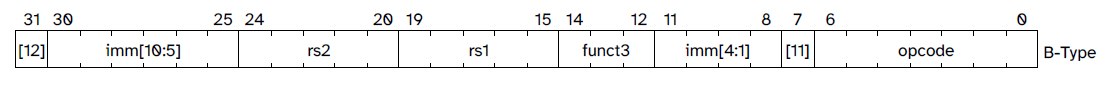
\includegraphics[width=0.95 \linewidth]{res/img/formato-b.png}
  \caption{Descripción del formato que deben seguir las instrucciones del tipo B}
\end{figure}

  \vspace{-0.2cm}
  \item \textbf{J}: saltos incondicionales. TODO: comentar diferencias con formato U
\end{itemize}